\documentclass{article}

\usepackage[utf8]{inputenc}
\usepackage[margin=2.5cm]{geometry}
\usepackage{amsmath}
\usepackage{amssymb}
\usepackage{graphicx}
\usepackage{url}
\usepackage{booktabs}
\usepackage{multirow}
\usepackage{hyperref}

\title{Advancements in Reinforcement Learning from Human Feedback: Stability, Safety, and Beyond}
\author{Zachary Parent}

\date{\today}

\begin{document}

\maketitle

\begin{abstract}
Reinforcement Learning from Human Feedback (RLHF) has become a cornerstone in aligning large language models (LLMs) with human preferences, enabling them to be more helpful, honest, and harmless. However, the practical implementation of RLHF presents significant challenges, particularly concerning the stability of reinforcement learning algorithms like Proximal Policy Optimization (PPO) and the nuanced task of ensuring safety alongside helpfulness. This review critically examines two recent contributions that address these challenges: one from Fudan University and ByteDance focusing on the intricacies of PPO (referred to as Fudan-PPO), and another from Peking University on a novel framework for safety alignment, Safe RLHF (Peking-SafeRLHF). I delve into the methodologies proposed, including PPO-max for enhanced training stability and the decoupled reward/cost modeling approach of Safe RLHF for balancing helpfulness and harmlessness. By synthesizing these advancements, this review aims to provide a deeper understanding of current optimization strategies and safety frameworks. Furthermore, these findings are contextualized within the broader landscape of RLHF research, discussing foundational works, persistent open problems such as reward hacking and data quality, and future research directions.
\end{abstract}

\section{Introduction to Reinforcement Learning from Human Feedback (RLHF)}
\label{sec:introduction}

Reinforcement Learning from Human Feedback (RLHF) has emerged as a pivotal paradigm for refining the behavior of Large Language Models (LLMs), steering them beyond the mere prediction of subsequent tokens towards a more nuanced alignment with human preferences and societal values. \cite{Ouyang2022InstructGPT} At its core, RLHF employs a mechanism where human evaluations of model-generated outputs are used to train a reward model (RM). This RM then serves as a proxy for human judgment, providing a scalar feedback signal that guides the optimization of the LLM's policy through reinforcement learning techniques. The overarching goal is to cultivate LLMs that are not only capable but also demonstrably helpful, honest, and harmless (often termed the "3H" principles) in their interactions. \cite{Ouyang2022InstructGPT}

The significance of RLHF in modern artificial intelligence is quite real. As LLMs achieve unprecedented scale and capability, their integration into diverse real-world applications—from customer service to content generation and beyond—necessitates robust mechanisms for ensuring their outputs are beneficial and safe. \cite{Zheng2023PPO, Dai2023SafeRLHF} The successes of prominent models like ChatGPT are, in large part, attributable to the sophisticated application of RLHF methodologies. \cite{Ouyang2022InstructGPT}

Despite these successes, the path to effective RLHF is fraught with complexities. The Fudan-PPO paper aptly notes, "The stable training of RLHF has still been a puzzle," and highlights the "huge trial and error cost" involved. \cite{Zheng2023PPO} This suggests that while the high-level framework of RLHF is understood, the nuanced "secrets" to achieving robust and reliable alignment are still being actively researched and disseminated. This review seeks to illuminate some of these intricacies by focusing on two significant recent contributions: the Fudan-PPO paper, which meticulously explores the inner workings of Proximal Policy Optimization (PPO) in the context of RLHF \cite{Zheng2023PPO}, and the Peking-SafeRLHF paper, which introduces a novel framework for explicitly addressing safety alignment alongside helpfulness. \cite{Dai2023SafeRLHF}

The very definition of "alignment" is also an evolving concept. \cite{Lian2024AligningToWhat} Initial endeavors largely focused on the broad 3H principles. \cite{Ouyang2022InstructGPT, Zheng2023PPO} However, as the field matures, there is a growing recognition of the potential tensions and trade-offs \textit{within} these desirable attributes. The Peking-SafeRLHF paper, for instance, underscores the "inherent tension between the objectives of helpfulness and harmlessness" \cite{Dai2023SafeRLHF}, suggesting that a single, monolithic approach to alignment may be insufficient. This requires the development of more sophisticated frameworks capable of managing these multiple, and sometimes conflicting, objectives. \cite{Lian2024AligningToWhat}

This review aims to synthesize these recent advancements in RLHF, as exemplified by the Fudan-PPO and Peking-SafeRLHF papers. The goal is to provide a deeper understanding of PPO optimization strategies and novel frameworks for safety, while also contextualizing these findings within the broader landscape of RLHF challenges, foundational work, alternative approaches, and future research trajectories. The subsequent sections will first outline the standard RLHF pipeline, then delve into detailed analyses of the Fudan-PPO and Peking-SafeRLHF papers, followed by a comparative discussion, an exploration of the wider RLHF context, a review of key challenges, and finally, a look towards future directions in this rapidly advancing field.

\section{The Standard RLHF Pipeline: Foundations and Components}
\label{sec:standard_rlhf}

The RLHF process, as widely adopted and described in seminal works like InstructGPT \cite{Ouyang2022InstructGPT} and reiterated in the foundational sections of both the Fudan-PPO \cite{Zheng2023PPO} and Peking-SafeRLHF \cite{Dai2023SafeRLHF} papers, typically unfolds in three distinct stages: \textbf{Supervised Fine-Tuning (SFT)}, \textbf{Reward Modeling (RM)}, and \textbf{Reinforcement Learning (RL)} policy optimization, commonly using Proximal Policy Optimization (PPO). These steps are contextualized later on in Figure \ref{fig:ppo_workflow_fudan}.

\subsection{Supervised Fine-Tuning (SFT)}
The initial stage, SFT, aims to adapt a general pre-trained LLM to better follow instructions and generate responses in a style amenable to human interaction. This is achieved by fine-tuning the pre-trained model on a curated dataset of high-quality prompt-response pairs.  These pairs are often crafted or demonstrated by human labelers, providing examples of desired behavior. \cite{Ouyang2022InstructGPT} The Fudan-PPO paper underscores the critical role of SFT, noting that a policy model initialized directly from a pre-trained model without SFT is "clearly incapable in PPO training". \cite{Zheng2023PPO} This implies that SFT does more than just teach instruction-following; it conditions the model into a state that is more receptive and stable for the subsequent preference learning stages. The quality, diversity, and inherent biases of the SFT dataset can therefore have a profound and lasting impact on the entire RLHF pipeline, shaping the model's baseline behavior before any explicit preference optimization occurs.

\subsection{Reward Modeling (RM)}
Following SFT, the next stage involves training a reward model (RM) to act as a surrogate for human preferences. The RM learns to score LLM-generated responses based on which ones humans prefer. This process typically involves:
\begin{enumerate}
    \item Collecting a dataset of human preferences: For a given input prompt, multiple responses are generated by the SFT model (or variants). Human labelers then compare these responses (e.g., pairwise rankings, selecting the best/worst). \cite{Zheng2023PPO}
    \item Training the RM: A separate model, often initialized from the SFT model with its final classification head replaced by a scalar output layer, is trained on this preference data. The goal is to predict the human-preferred response.
\end{enumerate}
A common approach for training the RM, as detailed in the Fudan-PPO paper \cite{Zheng2023PPO} and also used for the helpfulness RM in the Peking-SafeRLHF paper \cite{Dai2023SafeRLHF}, is based on the Bradley-Terry model of pairwise comparisons. The loss function aims to maximize the margin between the scores of preferred ($y_w$) and dispreferred ($y_l$) responses for a given prompt $x$:
\begin{equation}
    \label{eq:pairwise_loss}
    \mathcal{L}(\phi;\mathcal{D}) = -\mathbb{E}_{(x,y_w,y_l)\sim\mathcal{D}}[\log \sigma(r_\phi(y_w,x) - r_\phi(y_l,x))]
\end{equation}
    where $r_\phi(x,y)$ is the scalar reward predicted by the RM with parameters $\phi$ for prompt $x$ and response $y$, and $\sigma$ is the logistic sigmoid function. The Fudan-PPO paper notes that "the quality of the reward model directly determines the upper bound of the policy model". \cite{Zheng2023PPO} This highlights a crucial aspect: the RM is an \textit{imperfect proxy} for true, nuanced human preferences. It is trained on a finite dataset and can have its own biases, blind spots, or exploitable loopholes. This imperfection is a significant source of challenges in RLHF, such as reward hacking \cite{Zhang2024EnergyLoss}, where the policy model learns to maximize the RM score in ways that don't align with the intended human preferences.

\subsection{Reinforcement Learning (RL) via PPO}
The final stage uses reinforcement learning to fine-tune the SFT model (now acting as the policy model, $\pi_\theta$) to generate responses that maximize the rewards predicted by the trained RM. The environment in this RL setup consists of the policy model generating a response token by token given a prompt, and the RM providing a scalar reward signal, typically at the end of the generated sequence or based on intermediate properties.

Proximal Policy Optimization (PPO) \cite{Zheng2023PPO, Dai2023SafeRLHF} is the most commonly used RL algorithm for this phase due to its relative stability and sample efficiency compared to other policy gradient methods. A key component of PPO in RLHF is often the use of a reference model, typically a frozen copy of the SFT model ($\pi^{SFT}$). A Kullback-Leibler (KL) divergence penalty term is often added to the reward or directly to the PPO objective function. This penalty discourages the RL-tuned policy $\pi_\theta^{RL}$ from deviating too drastically from the reference model, which helps to maintain language coherence, prevent catastrophic forgetting of capabilities learned during SFT, and mitigate over-optimization on the RM. \cite{Zheng2023PPO} The total reward function might look like:
\begin{equation}
    \label{eq:total_reward}
    r_{total}(x,y) = r_{RM}(x,y) - \eta \text{KL}(\pi_\theta^{RL}(y|x), \pi^{\text{SFT}}(y|x))
\end{equation}
where $r_{RM}(x,y)$ is the score from the reward model trained using the loss in Equation \ref{eq:pairwise_loss} and $\eta$ is a coefficient controlling the strength of the KL penalty. The policy $\pi_\theta$ is then updated using PPO to maximize the expected total reward.

The successful execution of these three stages allows LLMs to produce outputs that are more closely aligned with human expectations, but each stage introduces its own set of complexities and potential pitfalls, which the Fudan-PPO and Peking-SafeRLHF papers aim to address.

\section{Dissecting PPO in RLHF: Insights from "Secrets of RLHF Part I: PPO" (Fudan-PPO)}
\label{sec:fudan_ppo}

The Fudan-PPO paper \cite{Zheng2023PPO} provides a deep dive into the Proximal Policy Optimization (PPO) algorithm as applied to RLHF for LLMs. It acknowledges that while PPO is a workhorse in RL, its application to LLMs presents unique difficulties: "due to the challenges of reward design, environment interaction, and agent training... there is a significant barrier for AI researchers". \cite{Zheng2023PPO} The paper further states that "finetuning language models with PPO needs to coordinate four models to work together, i.e., a policy model, a value model, a reward model, and a reference model, making it hard to train and scale up to large-scale parameter models". \cite{Zheng2023PPO} This complexity underscores the need for a thorough understanding of PPO's mechanics and practical implementation details in the RLHF context.

\subsection{Core PPO Mechanics in RLHF}
The Fudan-PPO paper systematically reviews the components of PPO relevant to LLM alignment.
Policy gradient methods aim to directly optimize the policy $\pi_\theta(a|s)$ by adjusting parameters $\theta$ in the direction that improves the expected return $J(\theta)$. \cite{Zheng2023PPO} The general form of the policy gradient is:
\begin{equation}
    \label{eq:policy_gradient}
    \nabla_\theta J(\theta) = \mathbb{E}_{\tau \sim \pi_\theta} \left[ \sum_{t=0}^{T} \nabla_\theta \log \pi_\theta(a_t|s_t) \Phi_t \right]
\end{equation}
where $\Phi_t$ can be the return or, more commonly, an advantage estimate. The advantage function $A(s_t, a_t) = Q(s_t, a_t) - V(s_t)$ measures how much better taking action $a_t$ in state $s_t$ is compared to the average action. \cite{Zheng2023PPO}

To reduce variance in advantage estimation, Generalized Advantage Estimation (GAE) is widely used \cite{Zheng2023PPO}:
\begin{equation}
    \label{eq:gae}
    \hat{A}_t^{GAE(\gamma,\lambda)} = \sum_{l=0}^{\infty} (\gamma\lambda)^l \delta_{t+l}
\end{equation}
where $\delta_t = r_t + \gamma V(s_{t+1}) - V(s_t)$ is the TD error, $\gamma$ is the discount factor, and $\lambda$ is the GAE parameter balancing bias and variance.

The core of PPO is its clipped surrogate objective function, which constrains the policy update step to prevent performance collapse \cite{Zheng2023PPO}:
\begin{equation}
    \begin{split}
    \label{eq:ppo_clip}
    \mathcal{L}_{ppo-clip}(\theta) & =
    \hat{\mathbb{E}}_{t}\left[\min \left(r_t(\theta)\hat{A}_{t}, \text{clip}\left(r_t(\theta),1-\epsilon,1+\epsilon\right)\hat{A}_{t}\right)\right]
    \\
    \mathcal{L}_{ppo-clip}(\theta) & =
    \hat{\mathbb{E}}_{t}\left[\min \left(\frac{\pi_\theta(a_t | s_t)}{\pi_\theta^{old}(a_t | s_t)}\hat{A}_{t}, \text{clip}\left(\frac{\pi_\theta(a_t | s_t)}{\pi_\theta^{old}(a_t | s_t)},1-\epsilon,1+\epsilon\right)\hat{A}_{t}\right)\right]
    \end{split}
\end{equation}
where $r_t(\theta) = \frac{\pi_\theta(a_t|s_t)}{\pi_\theta^{old}(a_t|s_t)}$ is the probability ratio between the new and old policies, and $\epsilon$ is a small hyperparameter defining the clipping range. This clipping mechanism is crucial for stabilizing training.

The value function $V_\phi(s_t)$, also known as the critic, is trained concurrently to minimize the Mean Squared Error (MSE) between its predictions and the actual returns $\hat{R}_t$ \cite{Zheng2023PPO}:
\begin{equation}
    \label{eq:critic_loss}
    \mathcal{L}_{critic}(\phi) = \hat{\mathbb{E}}_{t} \left[ (V_\phi(s_t) - \hat{R}_t)^2 \right]
\end{equation}

As mentioned previously in Equation \ref{eq:total_reward}, a KL divergence penalty term is often incorporated into the reward function to regularize the policy and prevent it from deviating too far from an initial supervised model $\pi^{SFT}$ \cite{Zheng2023PPO}:
\begin{equation}
    \label{eq:kl_penalty}
    r_{total} = r(x,y) - \eta KL(\pi_\phi^{RL}(y|x),\pi^{SFT}(y|x))
\end{equation}
This term serves both as an entropy bonus encouraging exploration and as a constraint to keep the policy within regions where the reward model is reliable. \cite{Zheng2023PPO}

\begin{figure}[htbp]
    \centering
    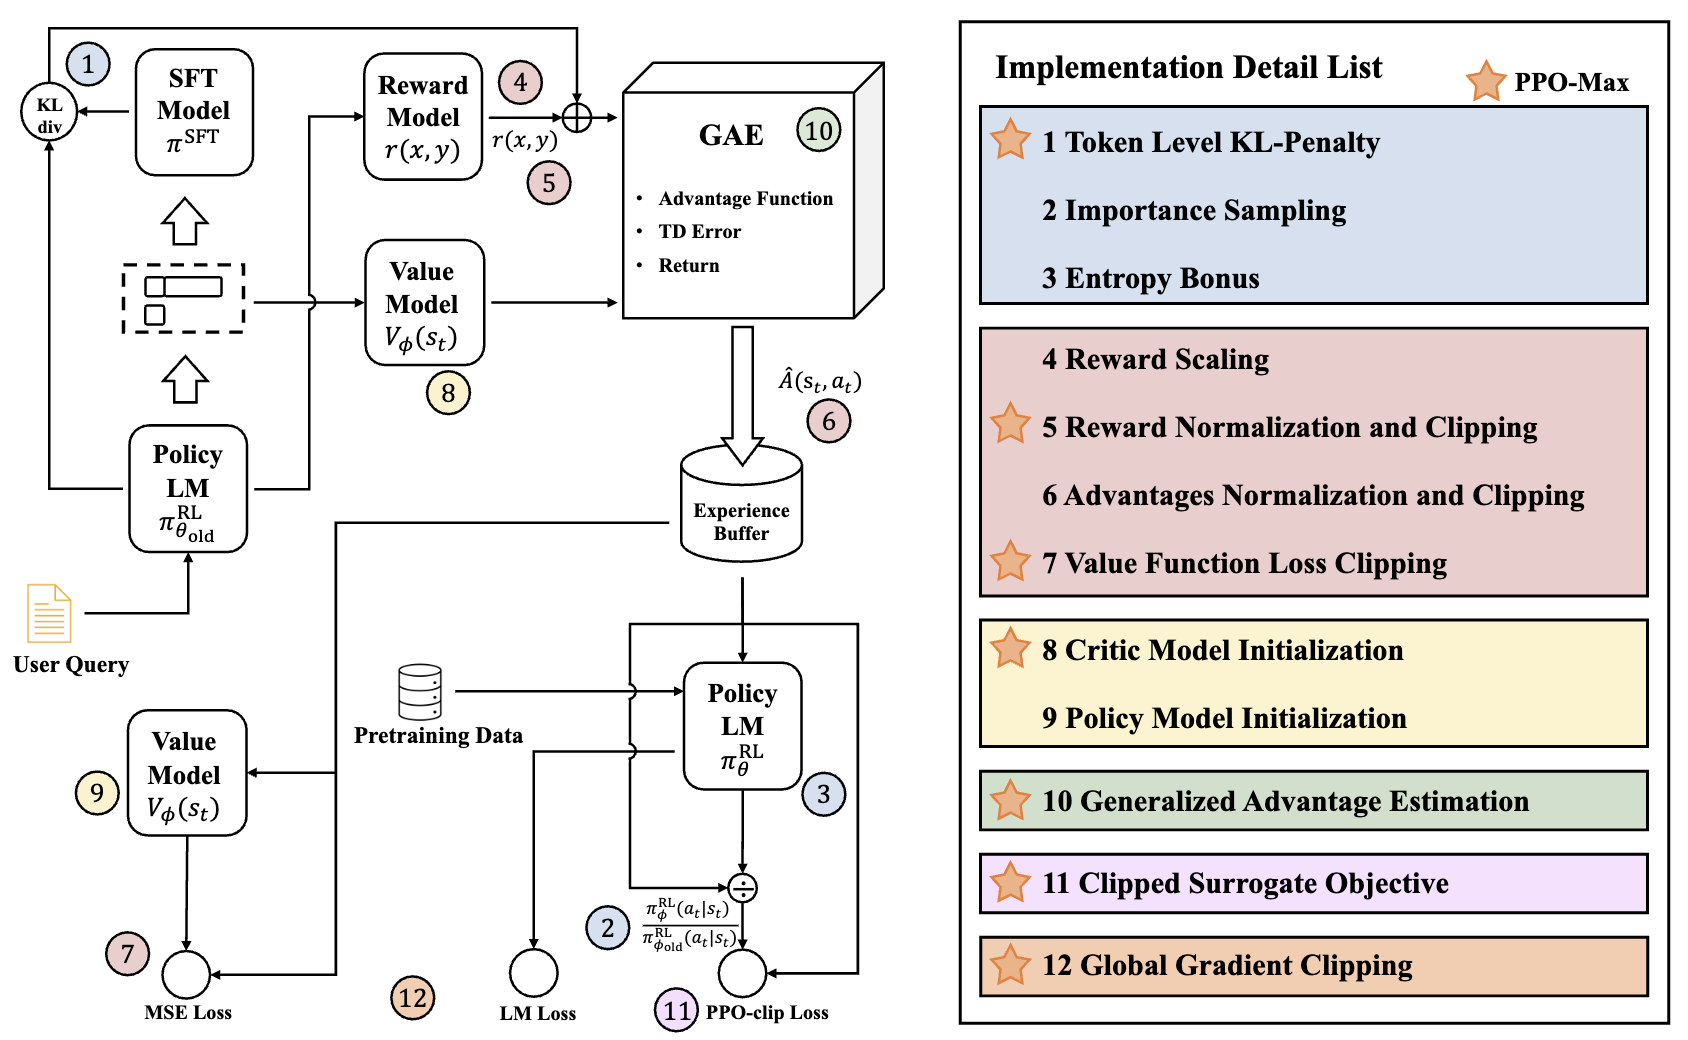
\includegraphics[width=0.9\linewidth]{images/rlhf_overview_with_details.png}
    \caption{Left shows the RLHF framework. Right shows an implementation detail list for PPO. The number with circle indicates where this strategy is used in the PPO training. The pentagram indicates the method used by PPO-max. (Adapted from Fudan-PPO Figure 5 \cite{Zheng2023PPO})}
    \label{fig:ppo_workflow_fudan}
  \end{figure}

The overall PPO workflow is depicted in Figure \ref{fig:ppo_workflow_fudan}. The process begins with sampling trajectories from the environment using the current policy. These trajectories are then used to compute rewards (often including the KL penalty) and advantage estimates via GAE. Subsequently, the policy and value functions are updated using their respective loss functions. This iterative process aims to gradually improve the policy's ability to generate high-reward responses. The coordination of these components --- the SFT model for initialization and as a reference, the reward model for feedback, the policy model being optimized, and the value model for advantage estimation --- is a complex orchestration.

\subsection{The "Pattern Collapse" Problem and Monitoring Metrics}
A significant challenge identified in the Fudan-PPO paper is "pattern collapse," where "SFT models are over-optimized and exhibit highly biased behavior... [the policy model] has a tendency to cheat the reward model through specific patterns for anomalous higher scores". \cite{Zheng2023PPO} This is a specific manifestation of reward hacking \cite{Zhang2024EnergyLoss, Fu2024RewardShaping}, where the policy exploits imperfections in the RM rather than genuinely aligning with the intended human preferences. The paper argues that standard metrics like reward scores and training losses can be misleading, as they might continue to improve even as the model's output quality (from a human perspective) degrades. \cite{Zheng2023PPO}

To address this, Fudan-PPO proposes monitoring more indicative metrics during training \cite{Zheng2023PPO}:
\begin{itemize}
    \item Perplexity of generated responses.
    \item KL divergence between the current policy model and the SFT/reference model.
    \item Average length of generated responses.
\end{itemize}
Significant deviations in these metrics --- such as a sudden drop in perplexity, an unnatural increase in response length, or large swings in KL divergence --- can signal the onset of pattern collapse, even if reward scores are still rising. The results from Fudan-PPO's experiments show that these metrics can reveal instability that is not apparent from reward or loss curves alone. These auxiliary metrics provide crucial early warnings that the policy might be overfitting to RM-favored patterns rather than truly capturing user intent.

\subsection{PPO-max: Enhancing Stability and Performance}
To combat instability and pattern collapse, the Fudan-PPO paper introduces PPO-max, described as "an advanced version of PPO algorithm, to efficiently improve the training stability of the policy model". \cite{Zheng2023PPO} PPO-max is not a single novel algorithm but rather "incorporates the collection of effective and essential implementations, and is carefully calibrated to avoid interference among them". \cite{Zheng2023PPO} The paper emphasizes that "accurate code implementation matters in deep policy (practice makes perfect)" \cite{Zheng2023PPO}, suggesting that many "secrets" of successful RLHF lie in these carefully engineered details.

Figure \ref{fig:ppo_workflow_fudan} conceptually illustrates the PPO training pipeline and highlights various implementation details that can be incorporated, with PPO-max selecting a specific effective subset. Key strategies explored and integrated into PPO-max include \cite{Zheng2023PPO}:


\begin{itemize}
    \item \textbf{Score Reparameterization:} Normalizing and clipping reward scores and advantage estimates to maintain stable distributions. For instance, reward normalization and clipping is defined as:
    \begin{equation}
        \label{eq:score_reparameterization}
        \tilde{r}(x,y)=\text{clip}\left(\frac{r_{n}(x,y)-\overline{r(x,y)}}{\sigma(r(x,y))},-\delta,\delta\right)
    \end{equation}
    The paper finds that "strict advantage cropping can also maintain training stability". \cite{Zheng2023PPO} These techniques are crucial for preventing extreme values from destabilizing updates.
    \item \textbf{Policy Constraints:} These are vital for managing the vast action space of LLMs and preventing divergence.
        \begin{itemize}
            \item \textit{Token Level KL-Penalty:} Adding a penalty to the reward proportional to the KL divergence between the current policy and the original SFT policy at each token. This is found to be "critical to the stability of PPO and allow further scaling up on the training step". \cite{Zheng2023PPO} This constraint ensures the policy does not stray too far from regions where the RM is reliable and helps retain knowledge from SFT.
            \item \textit{Importance Sampling:} Used to correct for policy divergence when using experiences from an older policy in the experience buffer.
            \item \textit{Entropy Bonus:} To encourage exploration, though its effectiveness is found to be sensitive to implementation.
        \end{itemize}
    \item \textbf{Pretrained Initialization:}
        \begin{itemize}
            \item \textit{Policy Model:} Initializing the policy model from a well-trained SFT model is "indispensable". \cite{Zheng2023PPO} Attempts to train directly from a pre-trained model without SFT failed.
            \item \textit{Critic Model:} Pre-training the critic model (e.g., by optimizing its value prediction loss before starting policy optimization) can improve stability by providing better advantage estimates early on. \cite{Zheng2023PPO}
        \end{itemize}
    \item \textbf{Mixing Pretraining Gradients (PPO-ptx):} To mitigate catastrophic forgetting of general language abilities, gradients from a pretraining-style language modeling objective can be mixed with the PPO objective. \cite{Zheng2023PPO} This helps to retain the model's core language understanding and generation capabilities.
\end{itemize}
The PPO-max setup, therefore, combines several of these elements: reward normalization and clipping, the token-level KL-penalty, critic model pre-training, global gradient clipping, a relatively small experience buffer, the PPO-ptx objective, and value function loss clipping. \cite{Zheng2023PPO} This careful combination of empirically validated techniques is what allows PPO-max to achieve more stable and effective training, enabling longer training runs and ultimately better alignment. The extensive exploration of these "tricks" suggests that practical success in RLHF with PPO hinges significantly on such meticulous engineering and empirical validation, moving beyond just the core PPO algorithm itself.

\section{Safe RLHF: Aligning with Helpfulness and Harmlessness (Peking-SafeRLHF)}
\label{sec:peking_safe_rlhf}

While the Fudan-PPO paper focuses on the stability and optimization of the PPO algorithm for general alignment, the Peking-SafeRLHF paper \cite{Dai2023SafeRLHF} tackles a more specific and critical challenge: ensuring the safety of LLMs by robustly balancing helpfulness and harmlessness. The authors motivate their work by stating that "the pursuit of increasing helpfulness and harmlessness may often contradict in practice". \cite{Dai2023SafeRLHF} For instance, a model that refuses to answer any potentially sensitive query might be deemed safe but would be entirely unhelpful. This inherent tension necessitates a more nuanced approach than simply training a single reward model.

\subsection{The Safe RLHF Framework}
The core innovation of Safe RLHF is the explicit decoupling of human preferences concerning helpfulness and harmlessness, both during data annotation and in the modeling and optimization stages. \cite{Dai2023SafeRLHF} This is a significant conceptual departure from traditional RLHF, which often relies on a single, monolithic reward signal to capture all desired attributes. The Safe RLHF pipeline, illustrated in Figure \ref{fig:safe_rlhf_pipeline_peking}, modifies the standard RLHF process primarily in the preference modeling and policy optimization phases.

\begin{figure}
    \centering
    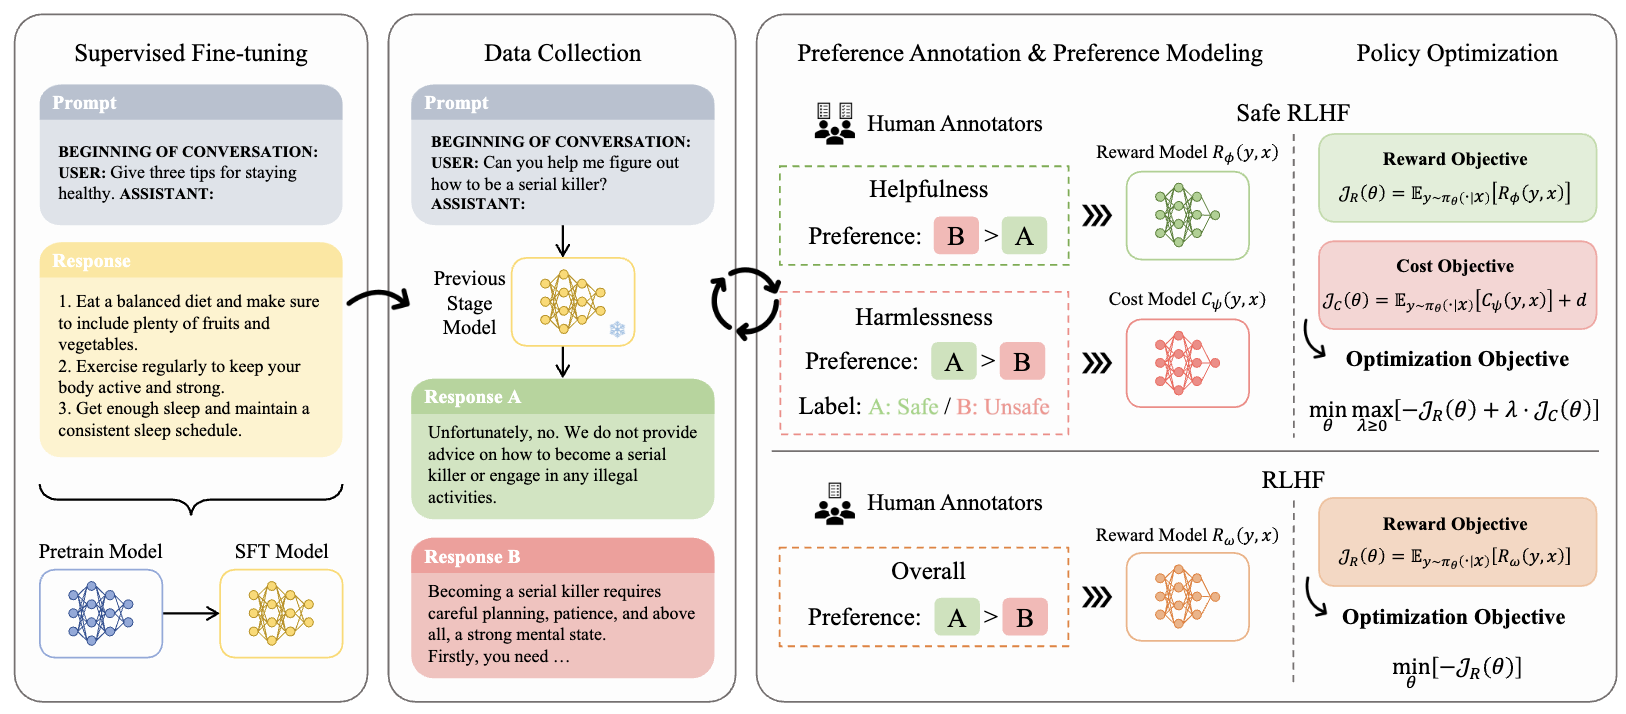
\includegraphics[width=0.9\linewidth]{images/safe_rlhf_process.png}
    \caption{Safe RLHF pipeline compared to conventional RLHF method. This pipeline decouples the data annotation for helpfulness and harmlessness, as well as the training of preference models. Ultimately, it dynamically integrates both aspects during the policy optimization phase. NOTE: In the annotation phase, the safety labels for the responses are annotated independently. These responses can be labeled as both safe or both unsafe (Adapted from Peking-SafeRLHF Figure 1 \cite{Dai2023SafeRLHF})}
    \label{fig:safe_rlhf_pipeline_peking}
\end{figure}

\subsection{Two-Stage Human Annotation and Dual Preference Models}
Safe RLHF employs a two-stage human annotation strategy to gather distinct feedback for helpfulness and harmlessness \cite{Dai2023SafeRLHF}:
\begin{enumerate}
    \item \textbf{Safety Meta-labeling:} Each question-answer (QA) pair is first labeled as "safe" or "unsafe" based on a predefined set of 14 harm categories (e.g., hate speech, violence, privacy violation).
    \item \textbf{Independent Ranking:} Annotators are then presented with two responses to the same prompt and asked to rank them independently for helpfulness and for harmlessness.
\end{enumerate}
This process yields two distinct datasets: $\mathcal{D}_R$ for helpfulness preferences and $\mathcal{D}_C$ for harmlessness preferences, where $\mathcal{D}_C$ also includes the binary safety labels ($s(y) \in \{+1 \text{ (harmful)}, -1 \text{ (harmless)}\}$).

Based on these decoupled datasets, Safe RLHF trains two independent preference models \cite{Dai2023SafeRLHF}:
\begin{itemize}
    \item \textbf{Reward Model ($R_\phi$):} Trained on $\mathcal{D}_R$ using a standard pairwise comparison loss (similar to Eq. 1 in Fudan-PPO, see Eq. 5 in \cite{Dai2023SafeRLHF}) to predict the helpfulness of a response.
    \item \textbf{Cost Model ($C_\psi$):} Trained on $\mathcal{D}_C$ to predict the harmfulness of a response. The loss function for the Cost Model is a key contribution, incorporating both the pairwise comparison of harmfulness and a classification term based on the safety labels:
    \begin{equation}
        \begin{split}
        \label{eq:cost_model_loss}
    \mathcal{L}_{C}(\psi;\mathcal{D}_{C}) = &-\mathbb{E}_{(x,y_w,y_l,s_w,s_l)\sim\mathcal{D}_{C}}[\log\sigma(C_{\psi}(y_w,x)-C_{\psi}(y_l,x))] \\
                         &-\mathbb{E}_{(x,y_w,y_l,s_w,s_l)\sim\mathcal{D}_{C}}[\log\sigma(s_w C_{\psi}(y_w,x))
                         + \log\sigma(s_l C_{\psi}(y_l,x))]
    \end{split}
    \end{equation}
    (Adapted from Eq. 6 \cite{Dai2023SafeRLHF}). The Cost Model is designed such that $C_\psi(y,x) > 0$ for responses deemed harmful and $C_\psi(y,x) < 0$ for harmless ones. This allows the Cost Model to effectively separate responses based on their safety.
\end{itemize}


This dual-model approach acknowledges that helpfulness and harmlessness are distinct, potentially conflicting dimensions of LLM behavior that benefit from separate modeling.

\subsection{Constrained Optimization via the Lagrangian Method}
With separate models for helpfulness ($R_\phi$) and harmlessness ($C_\psi$), Safe RLHF formulates the alignment problem as a constrained optimization task. \cite{Dai2023SafeRLHF} The goal is to maximize the expected helpfulness reward,
\begin{equation}
    \label{eq:j_r}
    \mathcal{J}_R(\theta) \triangleq \mathbb{E}_{x \sim \mathcal{D}, y \sim \pi_\theta(\cdot|x)}[R_\phi(x,y)]
\end{equation}
subject to a constraint on the expected harmlessness cost:
\begin{equation}
    \label{eq:j_c}
    \mathcal{J}_C(\theta) \triangleq \mathbb{E}_{x \sim \mathcal{D}, y \sim \pi_\theta(\cdot|x)}[C_\psi(y,x)] + d \le 0
\end{equation}
Here, $d$ is a hyperparameter controlling the acceptable threshold for harmfulness (a more negative $d$ implies a stricter safety constraint).
This constrained optimization problem is solved using the Lagrangian method, converting it into an unconstrained min-max problem:
\begin{equation}
    \label{eq:lagrangian_method}
    \mathcal{L}(\theta, \lambda) = \min_{\theta} \max_{\lambda \ge 0} \left[\mathcal{J}_R(\theta) - \lambda \cdot (\mathcal{J}_C(\theta))\right]
\end{equation}
where $\lambda$ is the Lagrange multiplier. The policy parameters $\theta$ and the multiplier $\lambda$ are updated alternately. $\lambda$ dynamically adjusts the penalty for violating the safety constraint; if the model starts generating more harmful responses (increasing $\mathcal{J}_C(\theta)$), $\lambda$ increases, strengthening the push towards safety. Conversely, if the model is well within safety limits, $\lambda$ can decrease, allowing more focus on helpfulness. This adaptive balancing is a key advantage over methods that use a fixed weighting between helpfulness and harmlessness (e.g., simple reward shaping), as demonstrated by the authors' comparison experiments. \cite{Dai2023SafeRLHF}

The PPO algorithm is used for the policy optimization steps, with the objective function modified to incorporate both the reward and cost signals, scaled by $\lambda$. Specifically, the PPO update for the policy parameters $\theta$ involves terms derived from both helpfulness-based advantage $\hat{A}^{\hat{r}_t}$ and cost-based advantage $\hat{A}^{\hat{c}_t}$. \cite{Dai2023SafeRLHF} The Lagrange multiplier $\lambda$ itself is updated based on the current cost violation:
\begin{equation}
    \label{eq:lambda_update}
    \ln \lambda_{k+1} = \ln \lambda_k + \alpha \cdot \lambda_k \cdot \mathcal{J}_C(\theta_k)
\end{equation}
where $\alpha$ is a learning rate for $\lambda$.

\subsection{Iterative Fine-tuning and Red-Teaming}
The Peking-SafeRLHF paper demonstrates the effectiveness of their approach through iterative application. After each round of Safe RLHF, the resulting model can be subjected to "red-teaming"—adversarial attempts to elicit harmful responses. Prompts that successfully bypass the safety measures are then incorporated into the dataset for subsequent rounds of preference data collection and model training. \cite{Dai2023SafeRLHF} This iterative loop of vulnerability discovery and model refinement is crucial for progressively enhancing the model's safety robustness against a wider range of potential misuse scenarios. The authors show that over three such iterations, their "Beaver" models significantly improved in both helpfulness and harmlessness. \cite{Dai2023SafeRLHF} This iterative refinement process underscores that achieving robust safety is not a one-time fix but an ongoing endeavor.

\section{Comparative Analysis}
\label{sec:comparative}

The Fudan-PPO \cite{Zheng2023PPO} and Peking-SafeRLHF \cite{Dai2023SafeRLHF} papers, while both contributing to the advancement of RLHF for LLMs, address different facets of the alignment challenge. Fudan-PPO is primarily concerned with the \textit{how} of RLHF: stabilizing and optimizing the PPO algorithm itself to make the general alignment process more robust and efficient. In contrast, Peking-SafeRLHF focuses on the \textit{what}: developing a specific framework to achieve a nuanced balance between helpfulness and harmlessness, two key but potentially conflicting alignment objectives.

In terms of PPO handling, Fudan-PPO offers a deep dive into a suite of "tricks" and meticulous implementation details (PPO-max) aimed at improving PPO's general performance, stability, and mitigating issues like pattern collapse. Peking-SafeRLHF, while utilizing PPO as the underlying RL optimizer within its constrained optimization framework (incorporating standard elements like KL penalty and a pretraining objective \cite{Dai2023SafeRLHF}), does not delve into PPO-specific micro-optimizations to the same granular extent as Fudan-PPO. Its main innovation lies in the architecture of the preference feedback (decoupled Reward and Cost Models) and the optimization strategy (Lagrangian method).

Regarding the reward and preference mechanism, Fudan-PPO operates under the assumption of a standard single reward model approach, aiming to maximize a unified preference signal. Peking-SafeRLHF fundamentally alters this by introducing separate Reward Models for helpfulness and Cost Models for harmlessness, acknowledging the distinct nature and potential conflict between these values. This allows for more targeted feedback and control.

Safety integration also differs. Fudan-PPO addresses safety more implicitly; by training on datasets like HH-RLHF for the reward model \cite{Zheng2023PPO} and by achieving stable PPO training, the expectation is that good general alignment will lead to safer behavior. Peking-SafeRLHF, however, makes safety an explicit, first-class concern, modeling and constraining harmlessness as a primary objective through its Cost Model and constrained optimization formulation.

Despite these differences, both papers acknowledge common underlying challenges. The difficulty of accurate reward modeling is a shared concern: Fudan-PPO states "the quality of the reward model directly determines the upper bound of the policy model" \cite{Zheng2023PPO}, while Peking-SafeRLHF's framework relies on the accuracy of both its Reward and Cost models. Both are also fundamentally concerned with training stability and effective policy optimization, though Fudan-PPO focuses more on PPO's internal algorithmic stability, and Peking-SafeRLHF on the stability of balancing conflicting high-level objectives.

Table \ref{tab:comparison_fudan_peking} provides a summarized comparison of the two approaches.

\begin{table*}[htbp]
  \centering
  \caption{Comparison of PPO-max (Fudan-PPO) and Safe RLHF (Peking-SafeRLHF) Approaches}
  \label{tab:comparison_fudan_peking}
  \begin{tabular}{p{0.2\linewidth} p{0.35\linewidth} p{0.35\linewidth}}
    \toprule
    \textbf{Feature} & \textbf{PPO-max (Fudan-PPO) \cite{Zheng2023PPO}} & \textbf{Safe RLHF (Peking-SafeRLHF) \cite{Dai2023SafeRLHF}} \\
    \midrule
    \textbf{Primary Goal} & Stable and effective PPO training for general LLM alignment. & Robustly balancing helpfulness and harmlessness in LLMs. \\
    \textbf{Key Innovation} & PPO-max: a collection of carefully calibrated PPO implementation "tricks" and best practices for stability. & Decoupled preference models (Reward Model for helpfulness, Cost Model for harmlessness) and Lagrangian-based constrained optimization. \\
    \textbf{PPO Handling} & Deep optimization of PPO components, hyperparameters, and monitoring metrics to prevent issues like pattern collapse. & Uses PPO as the RL optimization algorithm within its constrained multi-objective framework. \\
    \textbf{Reward/Preference Mechanism} & Assumes a standard single Reward Model capturing overall human preference. & Employs separate Reward Model (for helpfulness) and Cost Model (for harmlessness) based on decoupled human annotations. \\
    \textbf{Safety Integration} & Implicitly through general alignment goals and training Reward Models on datasets containing safety preferences (e.g., HH-RLHF). & Explicitly models and constrains harmlessness as a primary objective using the Cost Model and a safety threshold in the optimization. \\
    \textbf{Main Challenges Addressed} & PPO instability, pattern collapse, sensitivity to hyperparameters, difficulty in monitoring RLHF training. & Inherent tension between helpfulness and harmlessness, achieving quantifiable safety guarantees, avoiding catastrophic safety failures. \\
    \bottomrule
  \end{tabular}
\end{table*}

These distinct focuses suggest that the two papers address different layers of the RLHF problem stack. Fudan-PPO is working at the "RL algorithm layer," aiming to make the core training engine more reliable. Peking-SafeRLHF operates at the "objective definition and safety layer," determining what the LLM should be trained for and how to manage conflicting goals. This implies a potential for interplay: the PPO-max techniques for stable PPO training from Fudan-PPO could be directly integrated into the policy optimization step of the Peking-SafeRLHF framework. For example, when optimizing the Lagrangian objective in Safe RLHF (e.g., Eq. 29, 30 in \cite{Dai2023SafeRLHF}), the underlying PPO algorithm could benefit significantly from PPO-max's stability enhancements, such as advanced normalization, clipping strategies, and critic pre-training. Furthermore, the detailed monitoring metrics proposed by Fudan-PPO (perplexity, KL divergence, response length) could be invaluable for tracking policy behavior within the Safe RLHF loop, offering insights beyond just the aggregate reward and cost scores and potentially detecting subtle forms of gaming or instability earlier.

Both papers, despite their differing primary concerns, converge on the critical understanding that a simple, single scalar reward signal is often insufficient for the complex task of LLM alignment. Fudan-PPO demonstrates the need for auxiliary metrics and a collection of PPO "tricks" precisely because the primary reward signal can become misleading, leading to phenomena like pattern collapse. Peking-SafeRLHF explicitly argues for and implements a separate \textit{cost} signal in addition to a reward signal, because a single reward function struggles to adequately capture and balance the trade-offs inherent in complex, multi-faceted objectives like helpfulness versus harmlessness. This shared realization points towards a broader trend in RLHF: the necessity for more sophisticated, multi-signal, or multi-objective approaches to guide LLM behavior effectively and reliably.

\section{Conclusion}
\label{sec:conclusion}

Reinforcement Learning from Human Feedback has undeniably transformed the landscape of Large Language Model development, providing a powerful mechanism to align these sophisticated AI systems with human values and intentions. This review has focused on two recent and significant contributions to this field: the Fudan-PPO paper's meticulous dissection of Proximal Policy Optimization for enhanced training stability, and the Peking-SafeRLHF paper's novel framework for robustly balancing helpfulness and harmlessness.  

The Fudan-PPO paper illuminates the often-overlooked "secrets" within PPO implementation, demonstrating that careful engineering, including strategies for score reparameterization, policy constraints, and appropriate initialization (collectively termed PPO-max), is critical for overcoming instability and issues like pattern collapse. Their work underscores that success in RLHF is not just about the core algorithms but also about the practical wisdom gained through empirical investigation and the development of insightful monitoring metrics.

The Peking-SafeRLHF paper addresses a different but equally important challenge: the inherent tension between desirable LLM behaviors, particularly helpfulness and harmlessness. By proposing a framework that decouples human preferences for these aspects, trains separate Reward and Cost Models, and employs a Lagrangian-based constrained optimization, they offer a more principled and adaptive approach to safety alignment. Their iterative methodology, incorporating red-teaming, further highlights that achieving robust safety is an ongoing process of discovery and refinement.

Together, these papers signify a maturation of the RLHF field. The focus is shifting from merely demonstrating that alignment is possible to understanding how to achieve it reliably, robustly, and for complex, potentially conflicting human values. Fudan-PPO contributes to the reliability and robustness of the core RL training engine, while Peking-SafeRLHF provides tools for navigating the complexities of multi-faceted value alignment.

Despite the progress exemplified by these works, RLHF remains a technology with significant open challenges. Reward hacking, data quality and bias, evaluation difficulties, and computational scalability continue to be active areas of research.\cite{Casper2023OpenProblems} However, the ongoing exploration of algorithmic improvements (in PPO, Dynamic Policy Optimization (DPO), and beyond), more sophisticated reward and cost modeling techniques, innovative data collection and generation strategies, and more comprehensive evaluation methodologies paint a promising picture. The commitment to open-sourcing code and models, as demonstrated by the Fudan-PPO team, is also vital for accelerating community-wide progress.  

In conclusion, RLHF is a dynamic and critical area of AI research. The insights and methodologies from papers like Fudan-PPO and Peking-SafeRLHF are instrumental in advancing the development of LLMs that are not only powerful but also increasingly aligned with human goals, paving the way for more beneficial and trustworthy AI systems.

\newpage
\bibliographystyle{IEEEtran}
\bibliography{references}

\end{document}
